\documentclass{kththesis}
\usepackage{csquotes} % Recommended by biblatex
\usepackage[style=numeric,sorting=none,backend=biber]{biblatex}
\usepackage[swedish]{babel}
\usepackage{graphicx}

\addbibresource{references.bib} % The file containing our references, in BibTeX format

\title{Find objects in real estate images with convolutional neural networks}
\alttitle{Hitta object i fastighetsbilder med convolutional neural networks}
\author{Oskar Råhlén och Sacharias Sjöqvist}
\email{orahlen@kth.se och sacsjo@kth.se}
\supervisor{Handledare}
\examiner{Examinator}
\programme{Degree project in Computer Science}
\school{School of Electrical Engineering and Computer Science}
\date{\today}

% Uncomment the next line to include cover generated at https://intra.kth.se/kth-cover?l=en
% \kthcover{kth-cover.pdf}

\begin{document}
% Frontmatter includes the title-page, abstracts and table-of-contents
\frontmatter

\titlepage

\begin{abstract}
  English abstract goes here.
\end{abstract}

\begin{otherlanguage}{swedish}
  \begin{abstract}
    Svenskt sammanfattning
  \end{abstract}
\end{otherlanguage}

\tableofcontents

% Mainmatter is where the actual contents of the thesis goes
\mainmatter

% Citera med \texttt{} och \parencite{}

\chapter{Introduktion}

Just nu (april 2019) finns över 20 000 bostadsrätter (https://www.hemnet.se/statistik) till salu på Sveriges största mäklarsite (https://www.hemnet.se/om), där nästan hälften av dessa ligger i Stockholm. 
Dit kommer 2,8 miljoner (https://www.hemnet.se/om) unika besökare varje vecka och gör tillsammans över 2000 sökningar i minuten.
Detta ställer höga krav på filtreringsfunktionerna för att potentiella köpare snabbt ska kunna hitta sin drömbostad.
Idag erbjuds redan filtreringsfunktionerna ”antal rum”, ”boarea”, ”pris” samt ”område”. 
Det finns också en fritextsöka där man kan söka på vad mäklaren har skrivit i texten.
Exempel på sökord är ”balkong”, ”kakelugn” och ”sjöutsikt”. 

Problemet med att söka i mäklartexter är att det tvingar mäklaren att i texten nämna samtliga attribut som han eller hon vill göra sökbara. 
Detta gör att vissa attribut kan bli utelämnade vilket i sin tur gör fritextrutan sämre.

Exempelvis är det ofta självklart om det finns en balkong eller kakelugn på mäklarbilderna men det är inte alltid mäklaren väljer att skriva detta i den löpande texten.
Det hade därför varit intressant att utifrån mäklarbilderna automatiskt generera ett sökindex där varje bild knyts till ett antal attribut.
Dessa attribut skulle sedan kunna användas för att lägga till filtreringsalternativ i sökfunktionen och därmed skapa en bättre användarupplevelse.

Det skulle också gå att använda sig av denna metod för att knyta attribut såsom skick och typ av rum (Sovrum, badrum eller kök) till varje bild.
Kombinationen skulle göra sökningar såsom ”Kök i gott skick” möjligt.  

Denna data kan också vara användbar vid värdering av bostäder, då det enkelt skulle gå att jämföra priser på bostäder med olika attribut, tillexempel lägenheter med sköutsikt mot lägenheter utan sköutsikt eller lägenheter med ett kök i gott skick mot lägenheter med ett kök i sämre skick.

VET INTE RIKTIGT HUR JAG SKA FORMULERA MIG HÄR!! Känns Som ett halvbra stycke
För att på ett effektivt och precist sätt kunna knyta attribut till mäklarbilder behöver man använda sig av någon form av automatisk bildbehandling.
Detta går att göra med hjälp av maskininlärning och djupa neurala nätverk.
Sättet som detta görs på är att man tränar ett antal bilder som innehåller det givna attributet och ett antal som inte innehåller attributet.
Modellen tränas sedan med hjälpt av ett djupt neuralt nätverk. 
Efter varje träning så testas modellen för att mäta hur många träningar som krävs för bästa resultat.
När modellen är färdigtränad kan man använda denna genom att skicka in en bild som input och modellen berättar om bilden innhåller attributet eller inte.
 



  \section{Syfte}
  Syftet med denna studie är att titta på hur olika maskininlärningsmetoder kan användas för att hitta relevanta nyckelord till bilder på lägenhetsannonser. 
  

  \section{Frågeställning}
  Går det med nuvarande verktyg inom maskininlärning hitta attribut i bilder från lägenhetsannonser?


  \section{Avgränsningar}
  För att sätta en rimlig avgränsningar på denna uppsats kommer tre olika sorters attribut undersökas och jämföras med tre olika sorters deeplearningmodeller. 
  Attributen som kommer– användas är ”Balkong”, ”Kakelugn” samt ”Typ av rum” (Kök, badrum eller sovrum) och deelearningmodellerna som kommer användas är ”keras”, ”smartAI”, samt ”blabla”. 
  Anledningen till att flera attribut eller flera sorters modeller inte valdes är att det är resurskrävande att både samla in och sortera testdata samt att implementera modellerna. 
  Anledningen till att färre inte valdes var för att få spridning på attributen och modellerna, för kunna svara på om klassifiseringen fungerar i allmänhet och inte bara i enstaka testfall. 
  En annan avgräsning som gjort är att mäklarbilderna som används endast kommer från bostadsrätter, då det kan skilja sig ganska mycket på hur villor och bostadsrätter ser ut.

\chapter{Bakgrund}
  \section{Definitioner}
    \subsection{Mäklarbild}
    En mäklarbild är en bild tagen ämnad för att användas för försäljning av en fastighet. 

  \section{Maskininlärning}
  En maskininlärningsalgoritm är en algoritm som kan lära sig och bli bättre från data \parencite{Goodfellow-et-al-2016}. Det kan beskrivas som ett datorprogram som kan följa en grupp med uppgifter T och lära sig med hjälp av erfarenhet E och dess prestanda P är mätbar. Maskininlärning hjälper oss att läsa problem som är för svåra för program skrivna och designade av människor att lösa. 

  Enligt \cite{Goodfellow-et-al-2016} är ett vanligt problem att lösa med maskininlärning klassificeringsproblem. Det innebär att bestämma vilken av k klasser en viss indata tillhör. För att lösa detta skapar man vanligtvis en funktion som tar in indata x och returnerar y, vilket är ett tal som representerar klassen. Det går även att returnera en sannolikhetsdistribution över alla klasser. Enligt \cite{Goodfellow-et-al-2016} så löses modern objektigenkänning med djupinlärning.

  En typ av algoritmer inom maskininlärning är supervised learning algorithms \parencite{Goodfellow-et-al-2016}. En sådan algoritm lär sig av data (erfarenhet E) som redan är uppmärkt med rätt klass. Detta kallas för labeled data. Det man vanligtvis gör är att man delar upp den märkta datan i ett träningsset och testset. Därefter tränar man algoritmen på sitt träningsset och testar sedan hur bra den fungerar, i form av fel (error) eller noggrannhet (accuracy), på sitt testset.

  Enligt \parencite{Goodfellow-et-al-2016} så är så kallade AI-kompletta problem,som objektigenkänning, bra att ha en baseline modell som är baserad på djupinlärning. Det är även bra att börja med ett CNN om indata består av bilder. 

  Man borde använda någon form av regularization. Där är dropout bra och fungerar i många tillfällen. Early stopping borde nästan alltid användas. Batch normalization kan användas istället för dropout, för att minska generaliseringsfel. 

  Om problemet är studerat förut så kan det vara bra att utgå ifrån modeller och algoritmer som redan har visats sig fungera bra. I bildigenkänning så är det till och med vanligt att man utgår ifrån samma vikter, så kallad transfer learning. Vanligtvis tränas då CNN upp på bilder från ImageNet. 

    \subsection{Neural networks}
    Neurala nätverk är en modell inom maskininlärning. Dess mål är att approximera en funktion f \parencite{Goodfellow-et-al-2016}. De är en viktig del av maskininlärningen och en specifik typ av feedforward network är convolutional neural networks, som är vanligt förekommande inom bildkategorisering. 

    Den nuvarande tekniken för objektigenkänning använder sig huvudsakligen av maskininlärning \parencite{krizhevsky_imagenet_2012}. För att öka dess prestanda så kan man samla in mer data, lära sig mer kraftfulla modeller eller använda sig av bättre tekniker för att undvika overfitting.

  \section{Convolutional Neural Network}
  Convolutional Neural Network är en typ av nätverk för indata som kan ses som ett rutnät \parencite{Goodfellow-et-al-2016}. I fallet om bilder så är det ett tvådimensionellt rutnät av pixlar. Det som gör CNN speciellt är att de använder sig av den linjära operationen convolution istället för vanlig matrismultiplikation i minst ett av sina lager.

  För en så avancerad uppgift som objektigenkänning så räcker det inte med stora mängder data, det behövs en modell med tidigare erfarenhet (prior knowledge) som tar korrekta antaganden om bilder. Detta gör convolutional neural networks (CNNs) bra \parencite{krizhevsky_imagenet_2012}. Jämfört med ett vanligt feedforward neural network med samma storlek på varje lager, så har CNNs färre anslutningar och färre parametrar, vilket gör att de blir enklare att träna.


  

    \subsection{Arkitekturer}
    Ett bra sätt att välja arkitektur är att att testa flera olika arkitekturer och frysa alla lager förutom det sista, och se resultatet \parencite{Goodfellow-et-al-2016}. Efter man hittat den bästa så tränar man alla lager.

  \section{Transfer Learning}
  Transfer Learning handlar om att överföra information mellan två olika området \parencite{oquab_learning_2014}. I datorseende (computer vision) handlar transfer learning huvudsakligen om att minska träningsprocessen genom att använda ett neuralt nätverk som redan är tränat på andra kategorier av bilder. Så man överför vikterna från ett tränat nätverk till ett nytt nätverk och anpassar det sedan för att kategorisera det man anser att kategorisera.

  \section{Fine-tuning och minska overfitting}
  Enligt \cite{krizhevsky_imagenet_2012} finns det minst två bra tekniker för att minska overfitting, data augmentation och dropout.

    \subsection{Data Augmentation}

    \subsection{Dropout}

\chapter{Metod}
Detta kapitel kommer att beskriva metoden som användes för att ge mäklarbilder attribut.


\section{Datainsamling}
För att kunna träna modeller för de olika attributen ”balkong”, ”kakelugn” samt ”typ av rum” behövdes ett antal bilder som både uppfyllde dessa attribut samt ”negativa” bilder som inte uppfyllde dessa attribut.
Detta gjordes med ett pythonscript som heter Google Images Download (https://github.com/hardikvasa/google-images-download) och tar ett sökord, hur många bilder som ska laddas ner (X) samt från vilken källa bilderna ska hämtas från som input och ger tillbaka en mapp med de första X antal bilderna som hittas på Google från den givna källan. 

Bildkällan som valdes var https://hemnet.se då det är Sveriges största bostadsförmedlingssite med mängder av bilder.

Sökorden samt antalen som användes för detta beskrivs här:

\begin{center}
  \begin{tabular}{ |c|c|c| } 
   \hline
   Sökord & Antal \\ 
   \hline
   balkong hemnet & 400  \\ 
   \hline
   balkong vasastan & 400 \\ 
   \hline
   balkong inspiration & 400 \\ 
   \hline
   hemnet vardagsrum & 400  \\ 
   \hline
   hemnet badrum & 400 \\ 
   \hline
   Hemnet braskamin & 400  \\ 
   \hline
   hemnet öppen spis & 400 \\ 
   \hline
   vardagsrum braskamin & 400 \\ 
   \hline
   hemnet hall & 400 \\ 
   \hline
   hemnet kök & 400 \\ 
   \hline
   hemnet uteplats & 400   \\ 
   \hline 
  \end{tabular}
  \end{center}

Eftersom denna data inte är validerade mäklarbilder med det attribut som sökes påbörjades ett valideringsarbete där alla bilder manuellt validerades och sorterades enligt följande:
\begin{itemize}
  \item Alla bilder som inte uppfattades som mäklarbilder enligt definitionen ovan raderades
  \item Alla bilder som inte var tagna på lägenheter raderades
  \item Alla bilder med en eldstad las i en mapp med eldstäder
  \item Alla bilder med en balkong las i en mapp
  \item Alla bilder på ett kök las i en mapp
  \item Alla bilder på ett vardagsrum las i en mapp
  \item Alla bilder på ett badrum las i en mapp
  \item Negativa bilder skapades för samtliga mappar. Alltså skapades en mapp med bilder utan eldstad, en mapp med bilder utan balkong etc. Dessa skapades med hjälp av bilder i övriga mappar. 
\end{itemize} 

I varje mapp låg det slutligen runt 400 bilder. 

När detta var slutfört delades varje mapp i ytterligare två delar, en som kallades ”training” och en som kallades ”validation”.
I training palcerades de första 80\% av bilderna och i validation de sista 20\%.
Detta gjordes för att kunna testa hur modellerna presterade när de var färdigtränade med 20\% av den totala bildmassan.


\section{Modeller}
För att träna modellerna användes Python 3.6 med deeplearningramverket Pytorch 1.0.0. 
Modellerna tränades med  hjälp av pytorch i de olika ramverken ”Resnet”, ”Alexnet”, ”VGG-11”, ”Densenet” samt ”inception V3”.
Efter varje träningsrund (Epoch) kördes en validering för att se hur förbättringskurvan ser ut efter varje Epoch och när modellen börjar bli ”overfitted”.

Dessa modeller kördes ett antal epochs? och bla bla bla bla

\section{Uppföljning}
När modellerna var färdigtränade gjordes ett utdrag av statistik för att kunna jämföra modellerna sinsemellan.
Datan som hämtades för varje modell var


\section{Hårdvara}
Hårdvaran som användes när modellerna tränades var följande:

\subsection{Graphical processing unit (GPU)}
GPUn som användes var av modell Tesla K80 och hade tillgång till 128GB grafikminne.

\subsection{Central processing unit (CPU)}
CPUn som användes hade fyra kärnor 

\subsection{Random Access Memory (RAM)}
Det fanns tillgång till 61GB RAM-minne.


Hur vi gått tillväga. Vilka dataset, hur implementation gått till (verktyg, klassificerare, parametrar), hur vi valt features.
Hur evalueringen har gått till (traning, test, validation set).

Vi vill mäta både precision och recall. Plotta en PR curve.

Vi kan även plotta hur precisionen har gått om i förhållande till mer data, för att skapa en uppfattning av om modellen kan bli bättre med mer data. Vanligtvis gör man detta i log-skala \parencite{Goodfellow-et-al-2016}. 

Gör även att göra en grid search på hyperparametrar.

Hur vi kan använda oss av preprocessing kan vi  läsa i kapitel 12 av Goodfellow.

\chapter{Resultat}
Presentation av resultatet från våra olika tekniker och evalueringar. i tabeller och grafer. Även beräkningstid. 

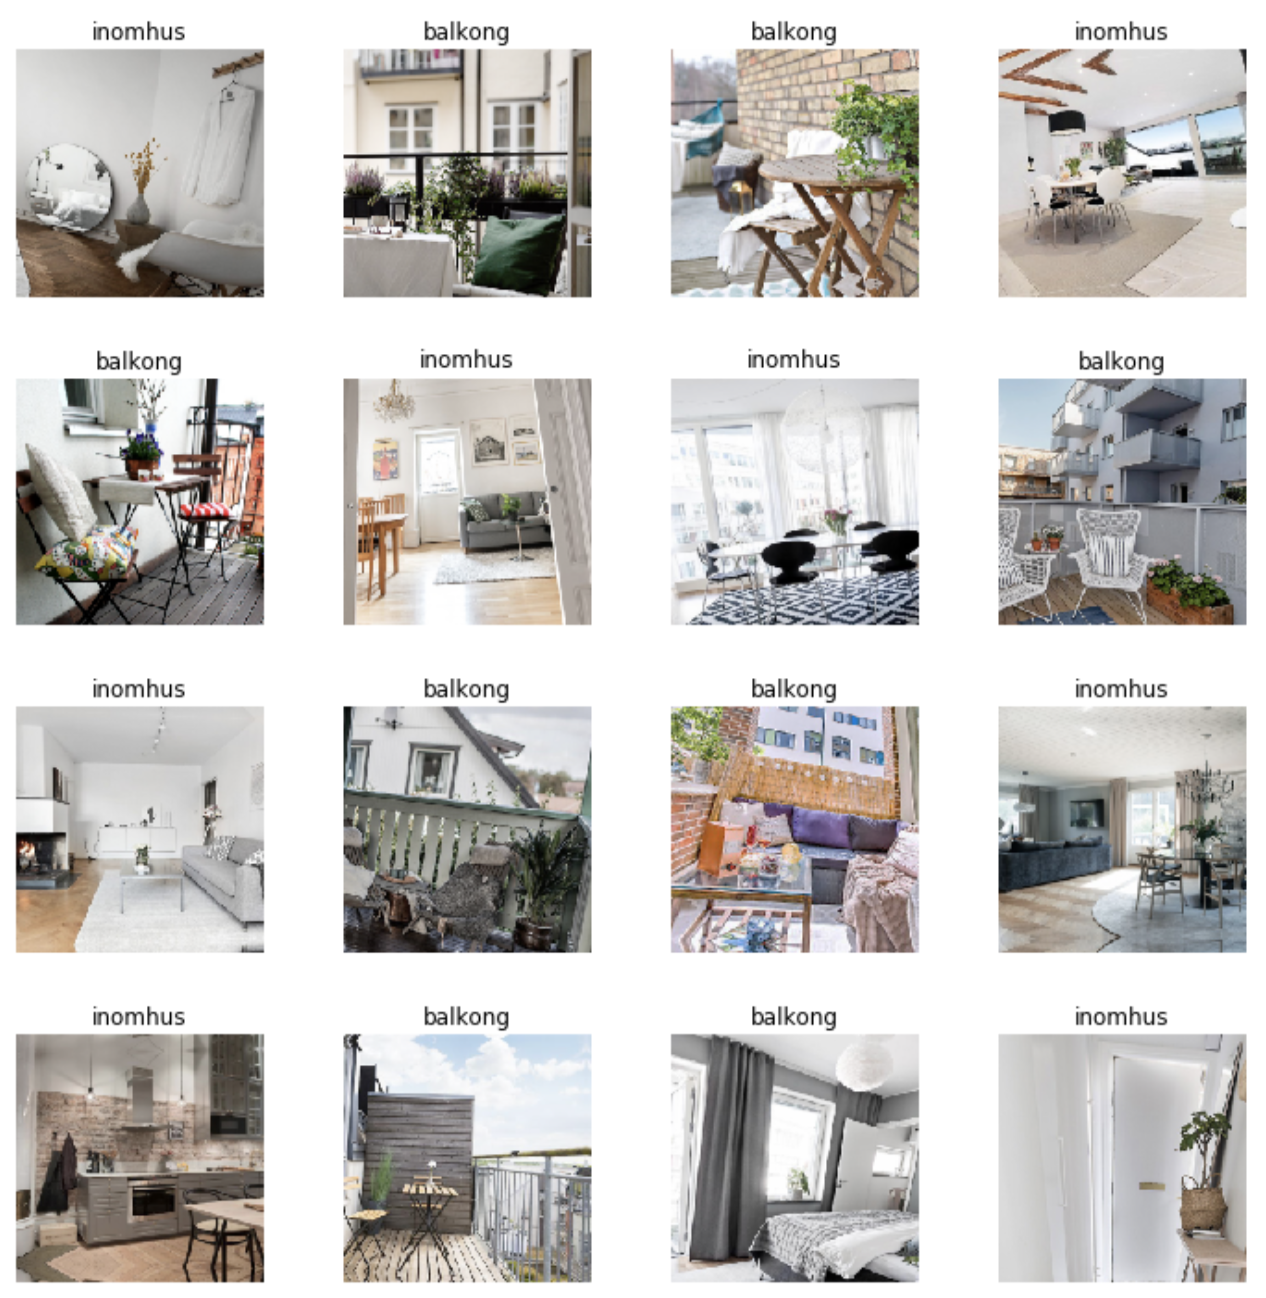
\includegraphics[width=10cm]{../images/1.png}

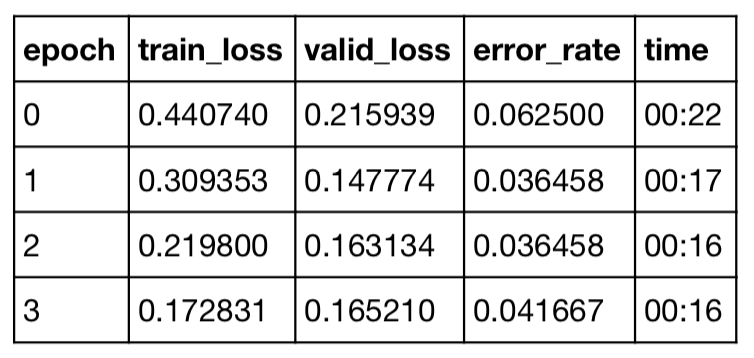
\includegraphics[width=10cm]{../images/2.png}

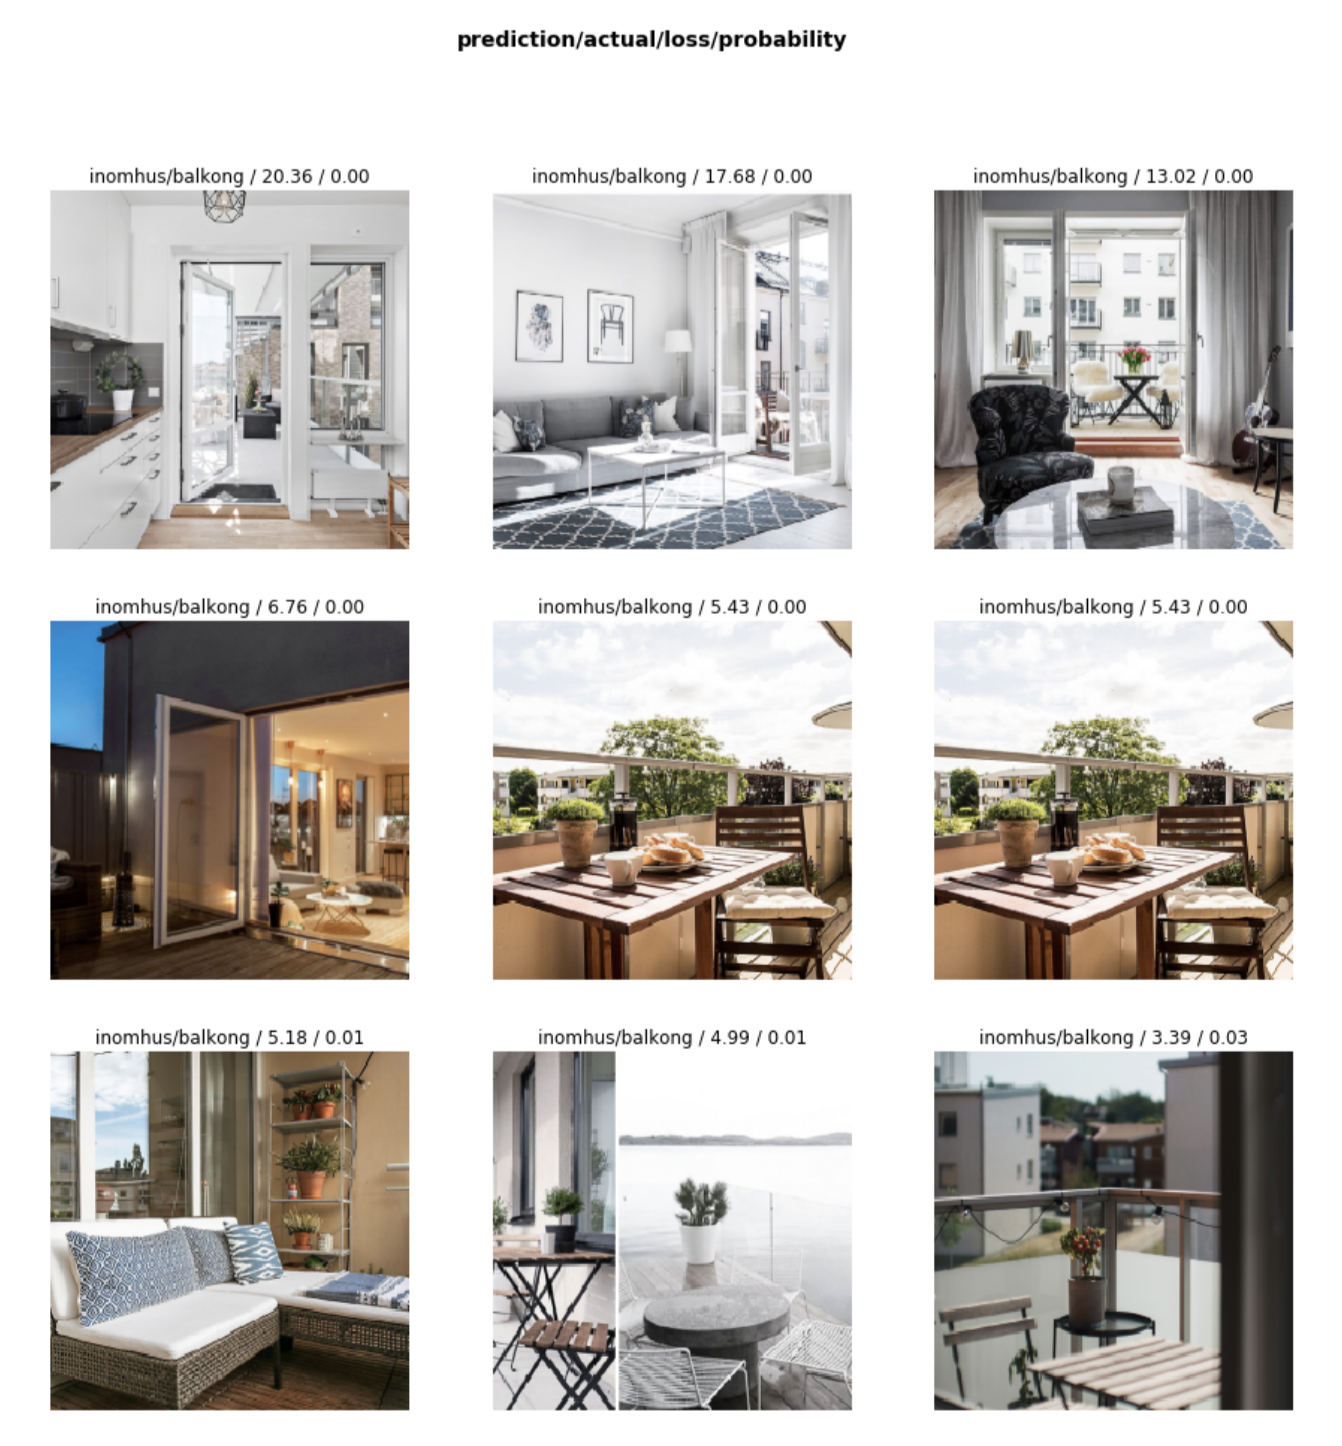
\includegraphics[width=10cm]{../images/3.png}

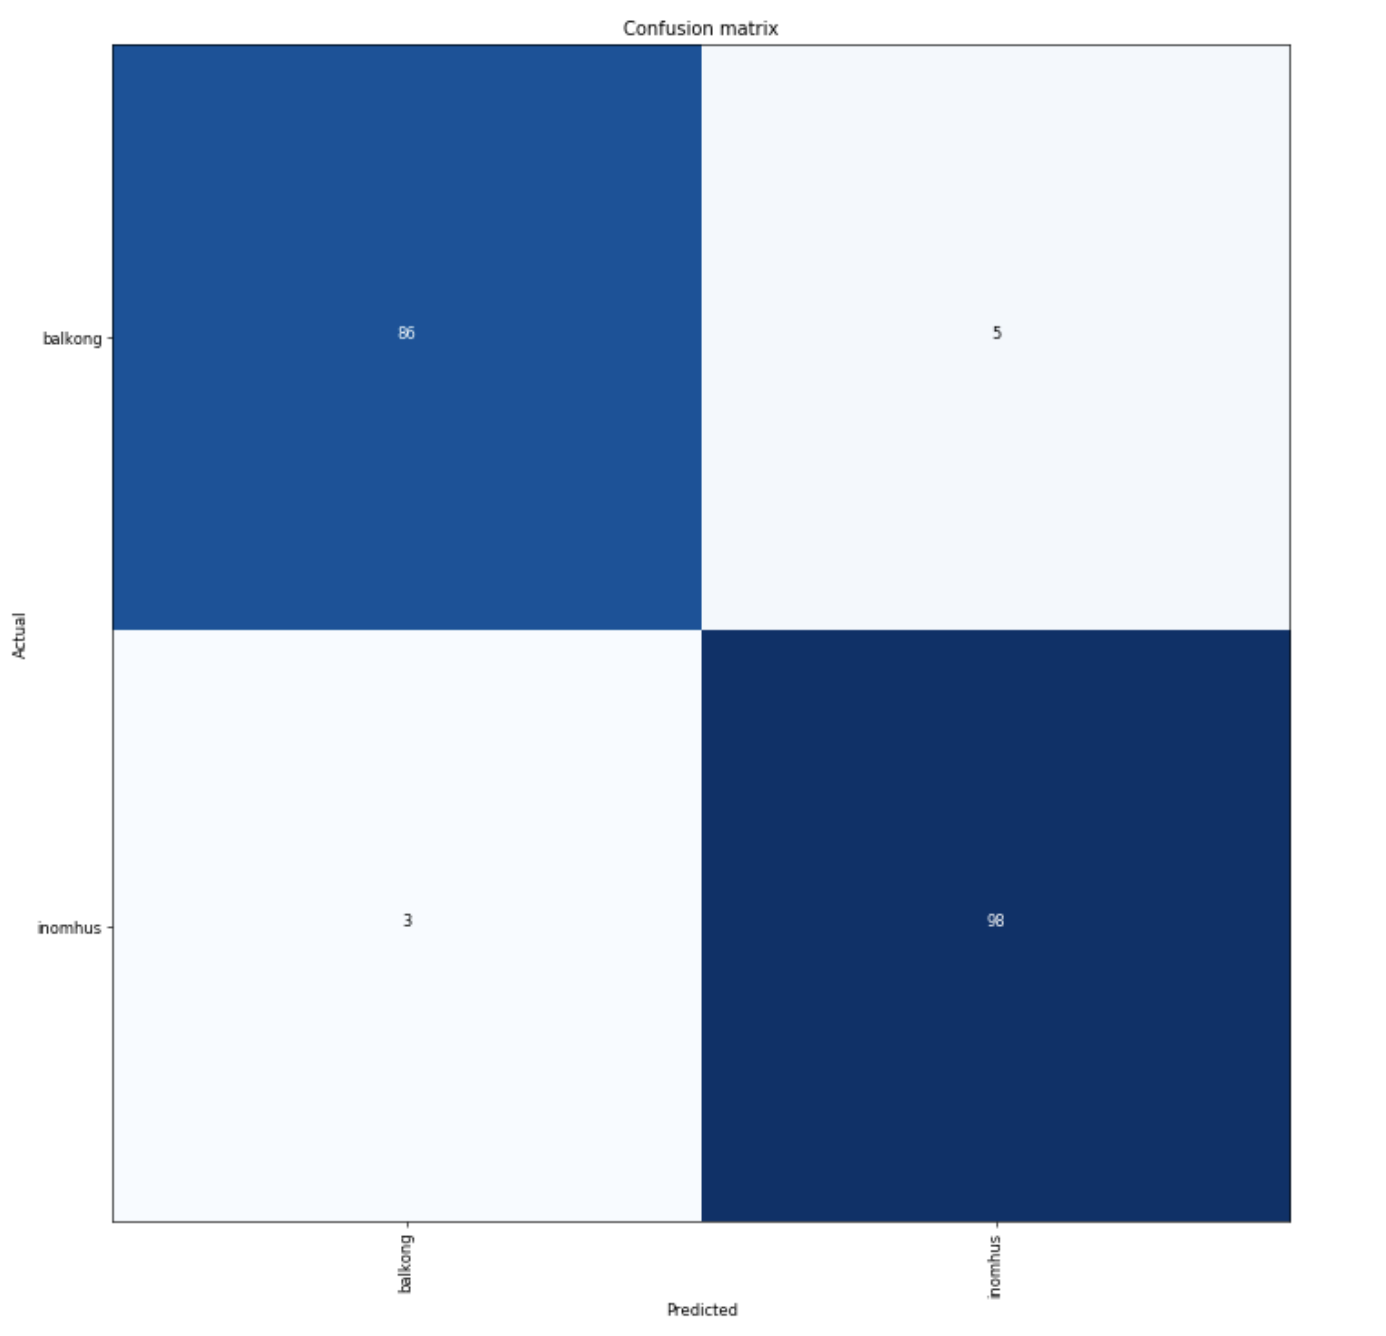
\includegraphics[width=10cm]{../images/4.png}

\chapter{Diskussion}
Diskutera resultatet och hur olika delar kan ha påverkat eller påverkade. Diskutera eventuell framtida forskning. Begränsningar med resultatet.
Etiska aspekter. Hållbarhet. 

  \section{Fortsätt forskning}
  Vid värdering så är det också intressant att få ut attribut, så kan man räkna med det i värderingskalkylen.

\chapter{Slutsats}  
Slutsats av vad vi kom fram till.

\printbibliography[heading=bibintoc]
\appendix
  \chapter{Appendix A}

\tailmatter
\end{document}
